
\chapter{The Large Hadron Collider and the ATLAS Detector}
\label{ch:LHCDetector}

This chapter describes the experimental details of the collider complex at the LHC and specifically the ATLAS detector used to produce, collect, and measure various particle properties.  The subsystems of the ATLAS detector are described in detail.
\section{The Large Hadron Collider}
\label{Section:LHC}
The LHC is the world's largest and most energetic particle accelerator.  As a hadron collider the LHC collides particles made up of quarks, typically proton-proton collisions.  Protons, as opposed to electrons/positrons at a previous collider such as LEP, have much higher mass and a significantly smaller amount of energy loss during acceleration due to synchrotron radiation (which scales as $\frac{1}{m^4}$).  Due to this the LHC is able to reach a much higher center of mass energy using the same circular ring used by LEP, though this higher energy comes at a cost.  Due to hadrons being made up of constituent partons (quarks and gluons), not all of which interact in any given collision, the particles that do not take place in the hard interaction are left over and create a 'messier' environment in the detectors.  This is opposed to lepton colliders, where all of the energy that goes into the collision is present in the final state particles coming from the interaction point.  The implication of this is that at hadron colliders the momentum along the beam axis cannot be known, only momentum in the transverse plane of a collision is known due to conservation of momentum.

\begin{figure}[ht!]
	\centering
	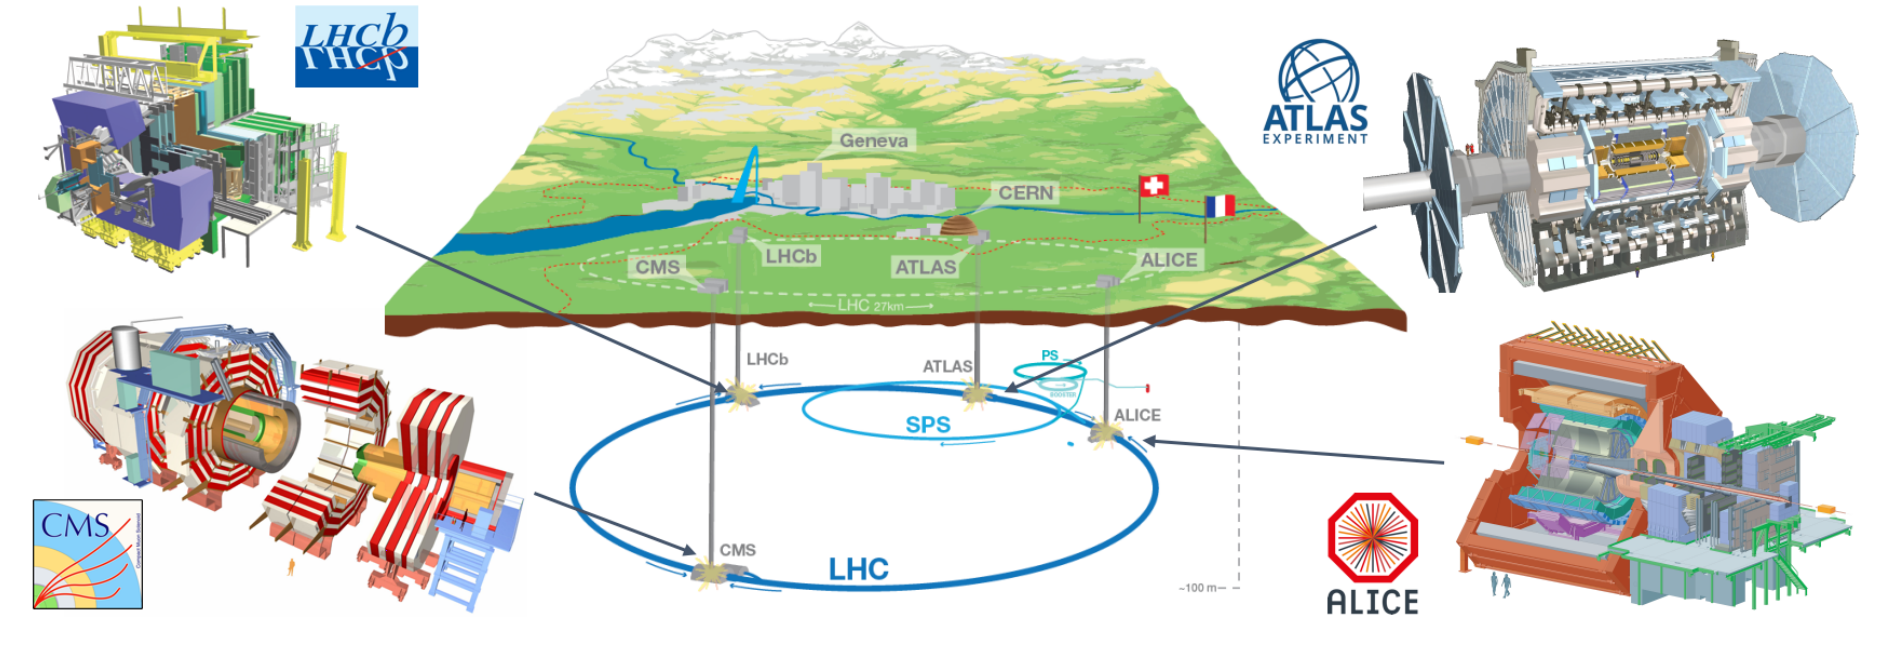
\includegraphics[width=\columnwidth]{../ThesisImages/LHCImages/LHCDetecPlacement.png}
	\caption[Map of LHC and the various detector experiments: ATLAS, CMS, LHCb, and ALICE located under the Franco-Swiss border near Geneva.]{Map of LHC and the various detector experiments: ATLAS, CMS, LHCb, and ALICE  located under the Franco-Swiss border near Geneva\cite{ATLASCoords}.}
	\label{fig:LHCDetPlace}
\end{figure}

The LHC is housed in a 27 kilometer ring running beneath the Franco-Swiss border near Geneva, Switzerland, and accelerates beams of protons (ions) to a center of mass energy of 13 TeV (5 TeV) using two counterpropagating circular beams around the ring.  The particles are then collided at one of the four primary interaction points, each of which house a dedicated detector as shown in Figure \ref{fig:LHCDetPlace}. 

In addition to the LHC beam line the accelerator uses a series of smaller accelerators to increase the energy of the particles before being introduced into the LHC.  This accelerator complex is detailed in Figure \ref{fig:AcceleratorMap}.  The start of the accelerator chain, and source of LHC protons, is the Linear Accelerator 2 (LINAC 2, purple) where hydrogen gas is placed inside of an electric field that separates the protons and electrons.  The remaining protons are passed through radiofrequency (RF) cavities and accelerated to 50 MeV using electric fields which oscillate at a frequency specific to the distance between any two RF cavities.
\begin{figure}[ht!]
	\centering
	\includegraphics[width=\columnwidth]{../ThesisImages/LHCImages/AcceleratorComplex.png}
	\caption[Schematic of the CERN accelerator complex.]{Schematic of the CERN accelerator complex\cite{LHCAccComplex}.
	}
	\label{fig:AcceleratorMap}
\end{figure}

After leaving LINAC 2 the protons are injected into the Proton Synchrotron Booster (BOOSTER, light purple) and accelerated to 1.4 GeV before being passed to the Proton Synchrotron (PS, magenta) in two batches with a separation of 1.2 seconds.  The PS accelerates the protons to 25 GeV to be injected into the Super Proton Synchrotron (SPS, blue) in a series of four batches separated by 3.6 seconds and are accelerated to 450 GeV.  The SPS is the second largest accelerator in the complex.  After reaching the 450 GeV of the SPS the particles are split and injected into the LHC in opposing directions where they are further accelerated to a collision energy of 6.5 TeV per beam leading to a center of mass energy of 13 TeV for the LHC during Run-2.

The first proton-proton collisions were produced in the LHC in 2008 at the injection energy of the SPS, $\sqrt{s} =900$ GeV.  During testing a faulty electrical connection caused a magnet quench, or a sudden loss of superconductivity, to occur.  This broke the nearby magnets and caused a delay in operations until late 2009 when LHC Run-1 began at a collision energy of $\sqrt{s} = 7$ TeV and later raised to $\sqrt{s}=8$ TeV in 2012 to complete Run-1.  Various upgrade and repairs on the LHC occurred throughout the long shutdown between 2012-2015 where the center of mass energy was increased to the LHC Run-2 energy of $\sqrt{s} = 13$ TeV.

\subsection{LHC Magnets}
The energies achieved in the collisions are only possible due to the LHC magnets that bend and focus the colliding particles.  The LHC uses the most powerful magnet technology that can be produced on an industrial scale.  There are 1232 superconducting dipole magnets each being 15m in length, weighing over 35 tons, and producing uniform magnetic fields of up to 8.4 T.  The niobium-titanium cables must be cooled to 1.9 K and operate with a current of 11,800 A.  Of these 1232 magnets 1104 are used to bend the particles around the ring and the remaining 128 are used in the beam dump.  To achieve the same center of mass energy using standard non-superconducting magnets the 27 km LHC would instead have to be upwards of 120 km long.

Since the bunches of particles are charged they will naturally diverge while traveling if not focused.  To correct for this an additional 392 quadrupole magnets, 5-7m in length, are used to focus the beam.  These quadrupoles are used in pairs: one which focuses in the horizontal plane and defocuses in the vertical plane and the other which focuses in the vertical plane and defocuses in the horizontal plane.  Together these magnets keep the beam squeezed to a usable size.  All of these magnets have two aperatures, one for each of the counter-propagating beams.

\subsection{Luminosity}
The amount of data collected at collider experiments is determined not only by the center of mass energy of colliding particles but also the rate of events produced.  This rate is called the luminosity and can be determined by the square of the number of particles in each bunch (since any one in one bunch can interact with any one in the other), the time between bunches, and the cross section of the bunch (or probability of a collision).
\[ \mathcal{L}=\frac{1}{\sigma}\frac{dN}{dt} \]
For any given proton-proton pair the luminosity can be expressed as:
\[ \mathcal{L}=\frac{1}{4\pi \sigma_x \sigma_y} \]
and can be expanded for the whole beam with the inclusion of the number of protons per bunch ($N_1$ and $N_2$), the number of bunches ($N_b$), and the frequency at which the bunches overlap ($f$) to:
\[ \mathcal{L}=\frac{N_1 N_2 N_b f}{4 \pi \sigma_x \sigma_y} \]
which can be iterated over the running time of the LHC (the total time with beams of proper size and energy propagating through the LHC) giving the total delivered luminosity.  This total integrated luminosity as a function of time during LHC Run-2 is shown in Figure \ref{fig:ATLASLumi}.  This luminosity value can be mulitplied by the probability, or cross section, of any particular final state to obtain the number of times that final state is produced with a given luminosity.
\begin{figure}[ht!]
	\centering
	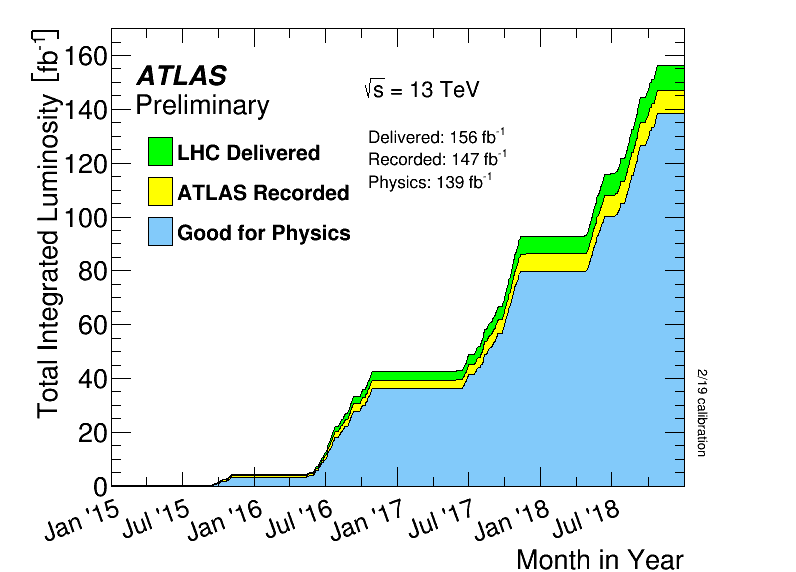
\includegraphics[width=.7\columnwidth]{../ThesisImages/LHCImages/ATLASLumi.png}
	\caption[Total integrated luminosity as a function of time delivered by the LHC(green), recorded (yellow) and declared good for physics analysis (blue) by the ATLAS detector throughout Run 2 consisting entirely of 13 TeV $pp$ collisions.]{Total integrated luminosity as a function of time delivered by the LHC(green), recorded (yellow) and declared good for physics analysis (blue) by the ATLAS detector throughout Run 2 consisting entirely of 13 TeV $pp$ collisions\cite{ATLASLumi}.}
	\label{fig:ATLASLumi}
\end{figure}


\subsection{Pileup}

Increasing the luminosity is very beneficial for increasing the statistics needed when searching for rare events but it brings additional challenges as well.  Most interactions at any given detector are not hard-scatter events that correspond to poentially interesting physics cases but are instead soft collisions which create noise in the various detector experiments.  The LHC works hard to deliver as much data to the experiments as possible and delivers bunches of protons at a time.  It is possible for multiple pairs of protons to undergo these soft inelastic collisions at a time.  The average number of interactions per bunch crossing, or pileup $\langle{\mu}\rangle$, for Run-2 was 33.7, shown in Figure \ref{fig:ATLASmeanIntperCrossing}. 
\begin{figure}[ht!]
	\centering
	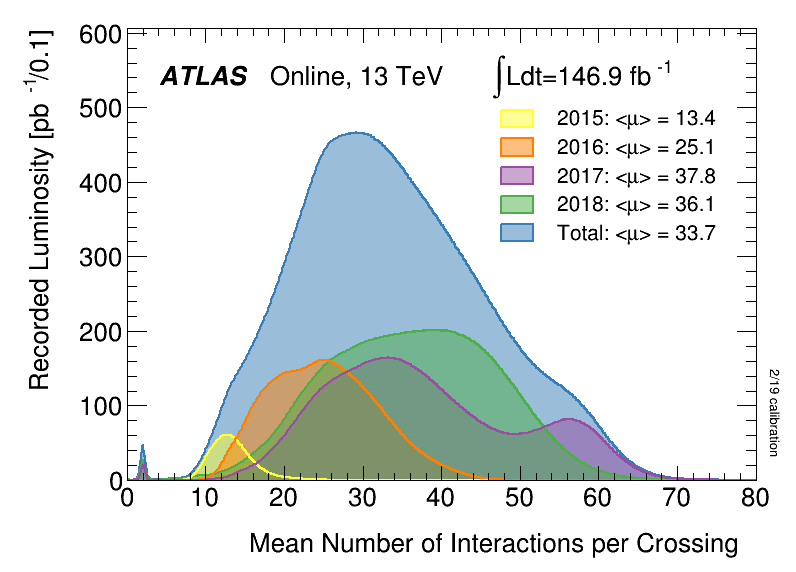
\includegraphics[width=.7\columnwidth]{../ThesisImages/LHCImages/meanIntperCrossing.png}
	\caption[Luminosity-weighted distribution of the mean number of interactions per bunch crossing for the entirety of Run 2 shown by individual years, 2015 (yellow), 2016(orange), 2017 (purple), 2018 (green), as well as an integrated total (blue).]{Luminosity-weighted distribution of the mean number of interactions per bunch crossing for the entirety of Run 2 shown by individual years, 2015 (yellow), 2016(orange), 2017 (purple), 2018 (green), as well as an integrated total (blue)\cite{ATLASLumi}.
	}
	\label{fig:ATLASmeanIntperCrossing}
\end{figure}
 The pileup must be accounted for when separating the tracks and energy deposited from an interesting hard-scatter event from the other soft collisions which occur at nearly the same time within a detector.  The difficulty of separating out one event from another can be seen in Figure \ref{fig:HighPileup} where there are 28 reconstructed verticies.  An extreme case of 65 reconstructed verticies is also shown in Figure \ref{fig:HighPileup2}.  As the LHC will continue to operate at higher and higher luminosities in the future, the amount of pileup that will need to be dealt with will continue to increase.  
\begin{figure}[ht!]
	\centering
	\includegraphics[width=.7\columnwidth]{../ThesisImages/LHCImages/28VertexPileup.png}
	\caption[A candidate dimuon event ($Z\rightarrow \mu^+ \mu^-$) with 28 reconstructed verticies collected in 2018 with the ATLAS detector.]{ A candidate dimuon event ($Z\rightarrow \mu^+ \mu^-$) with 28 reconstructed verticies collected in 2018 with the ATLAS detector\cite{ATLASLumi}.
	}
	\label{fig:HighPileup}
\end{figure}

\begin{figure}[ht!]
	\centering
	\includegraphics[width=.7\columnwidth]{../ThesisImages/LHCImages/65VertexPileup.png}
	\caption[A candidate dimuon event ($Z\rightarrow \mu^+ \mu^-$) with 65 reconstructed verticies collected in 2017 with the ATLAS detector.]{ A candidate dimuon event ($Z\rightarrow \mu^+ \mu^-$) with 65 reconstructed verticies collected in 2017 with the ATLAS detector\cite{ATLASLumi}.
	}
	\label{fig:HighPileup2}
\end{figure}

\section{The ATLAS Detector}
\label{sec:ATLAS}
The ATLAS dectector, depicted in Figure \ref{fig:ATLASOverview}, is one of the two general-purpose detectors at the LHC.  It is the largest detector of its kind ever built at 46 meters in length, 25 meters in diameter, weighing 7000 tons, and containing around 3000 kilometers of cables\cite{ATLAS}.  Around the interaction points within the detector the ATLAS detector covers nearly the entire solid angle and is nominally symmetric.  ATLAS is built up of a variety of concentric subsystems, which will be discussed throughout this section, each with a specialized task and optimized for the measurement of different particle signatures.  
\begin{figure}[ht!]
	\centering
	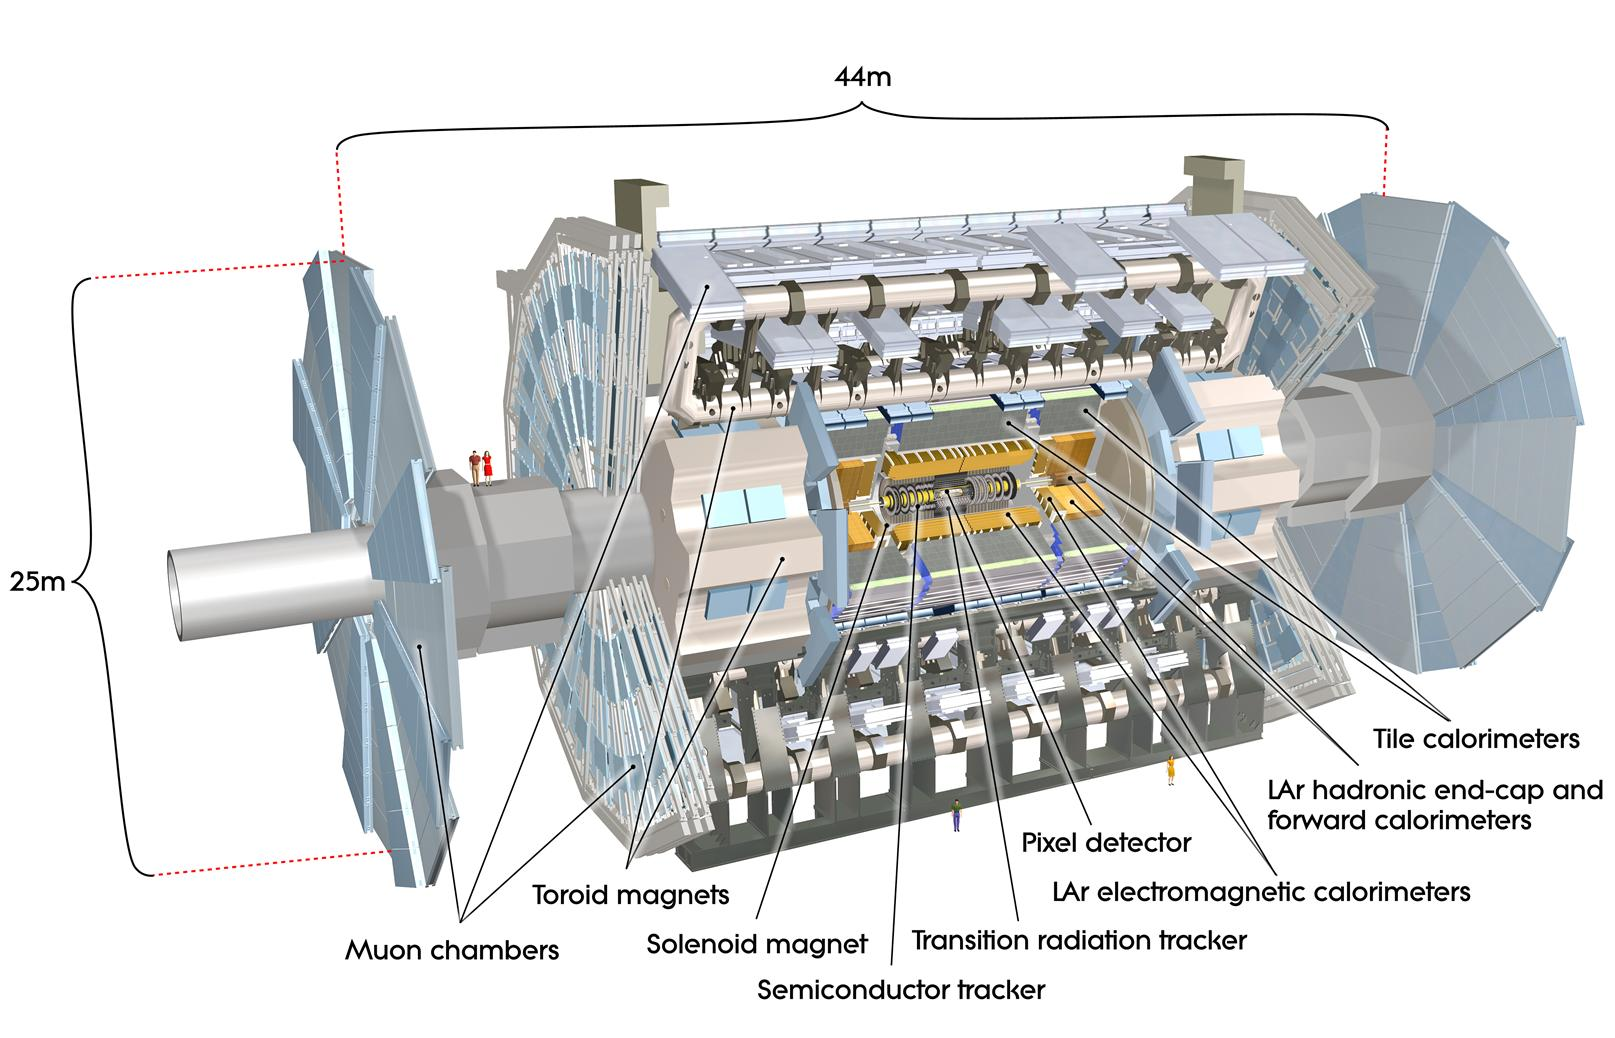
\includegraphics[width=\columnwidth]{../ThesisImages/LHCImages/AtlasDetector.png}
	\caption[Schematic of the ATLAS detector.]{Schematic of the ATLAS detector\cite{ATLAS}.
	}
	\label{fig:ATLASOverview}
\end{figure}
The primary subsystems used to measure particle trajectories and momenta accurately are the inner detector (Section \ref{sec:InnerDet}), the hadronic and electromagnetic calorimeters (Section \ref{sec:EMHCal}), and the muon system (Section \ref{sec:MuCal}).  The inner detector measures the paths of charged particles, called tracks.  The electromagnetic and hadronic calorimeters measure the energy of charged and neutral particles. The muon system measures the momenta of minimum ionizing particles (MIPs).  

In addition to the various detectors and calorimeters the ATLAS detector has a magnet system (Section \ref{sec:ATLASMagnet}) that bends charged particles in the detector, allowing for a measurement of their charge and momentum and distingushing them from neutral particles.  Between the inner detector and the calorimeters is a solenoid which provides an axial magnetic field.  Between the calorimeters and the muon system is a toroidal magnet, from which ATLAS got its original acronym (\textbf{A} \textbf{T}oroidal \textbf{L}HC \textbf{A}pparatu\textbf{S}).



\subsection{Common Detector Variables and the ATLAS Coordinate System}
The ATLAS detector uses a right-handed coordinate system with the origin at the interaction point.  In a Cartesian coordinate system the z-axis is defined to be along the beam pipe (positive towards LHC Point 8) while the x-axis points toward the center of the LHC ring which means the positive y-axis points upwards as shown in Figure \ref{fig:ATLASCoords}.  In practice coordinates used are a modified polar coordinate system.  In the transverse (xy-)plane to the beam line the azimuthal angle, $\phi$, is measured around the beam axis and radius, $r$, are used.  Away from the transverse plane the pseudorapidity, $\eta$, is defined by the polar angle (from the y-axis), $\theta$, to be $\eta= -\text{ln}[\text{tan}(\theta/2)]$.  Differences in $\eta$ are Lorentz invariant under longitudinal boosts such that the differences in the rest frames of colliding particles are not important for massless particles.  Since the particles typically present in the ATLAS detector are highly energetic, and therefore have a large boost, the pseudorapidity is a good estimate of the true rapidity of the particles.  Massless particles are also produced uniformly in $\eta$ and not in $\theta$  which is why $\eta$ is preferred.

\begin{figure}[ht!]
	\centering
	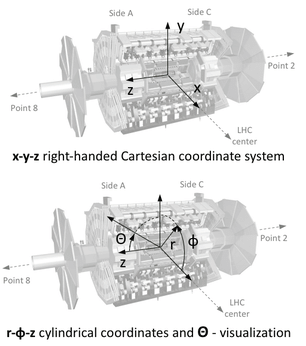
\includegraphics[width=0.5\columnwidth]{../ThesisImages/LHCImages/ATLASCoords.png}
	\caption[Coordinate system used in the ATLAS Collaboration.]{Coordinate system used in the ATLAS Collaboration\cite{ATLASCoords}.
	}
	\label{fig:ATLASCoords}
\end{figure}

The distance between any two objects within the ATLAS detector can be described geometrically by the variable $\Delta R = \sqrt{\Delta \eta^2 + \Delta \phi^2}$.  Another common variable used is the missing transverse energy, $E^{\text{miss}}_T$.  The information known about the missing energy is limited to the transverse plane because the momenta of the colliding particles is unknown along the beamline. 




\subsection{Magnet Setup}
\label{sec:ATLASMagnet}

The ATLAS detector has two magnet systems of note.  The first is the superconducting solenoid that surrounds the inner detector with a magnetic field aligned with the beam axis.  The solenoid has a magnetic field of 2T that makes the tracking of charged particles possible with the inner detector.  This magnet is a thin single layer coil, which is imperative to minimize the amount of material in front of the calorimeters. 

The toroid system consist of two parts, the end-cap and the barrel magnets.  The windings of these magnets is shown in Figure \ref{fig:ATLASMagnetWinding}.  Each of these magnets consist of eight superconducting air-core coils, together weighing 830 tons.  The end-cap coils are interleaved with the barrel coils.  A peak magnetic field strength of 3.9T (4.1T) is achieved in the barrel (end-cap) toroid which assists in the track and momentum measurement of high energy muons as they leave the ATLAS detector.  The barrel toroids cover a range of $|\eta|<1.4$ while the endcap toroids cover the range $1.6 < |\eta| <2.7$.  The remaining region is covered by a combination of the field of the two sets of toroids.
\begin{figure}[ht!]
	\centering
	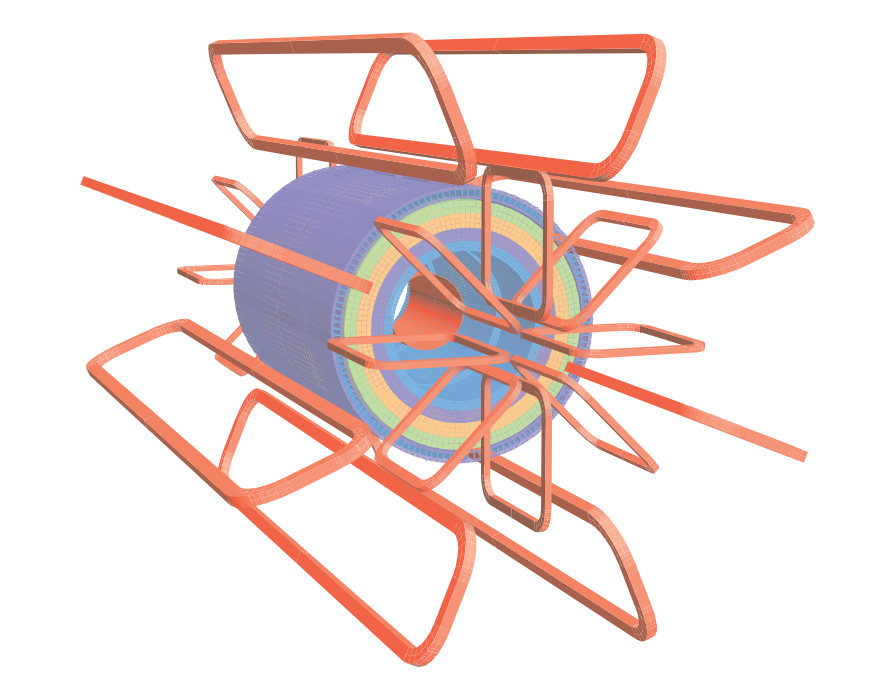
\includegraphics[width=0.7\columnwidth]{../ThesisImages/LHCImages/ATLASMagnetWinding.png}
	\caption[Schematic of the windings of the ATLAS magnet.]{Schematic of the windings of the ATLAS magnet\cite{ATLAS}.
	}
	\label{fig:ATLASMagnetWinding}
\end{figure}

%\subsection{SubDetectors}
\subsection{Inner Detector}
\label{sec:InnerDet}
The inner detector sits inside the solenoid magnet and is used to reconstruct charged particle tracks as they bend due to the magnetic field.  The inner detector is made up of four distinct parts.  The Insertable B-Layer (IBL) \cite{Capeans:1291633}, the Pixel Detectors, the Semiconductor Tracker (SCT), and the Transition Radiation Tracker (TRT)\cite{CERN-LHCC-97-016}.  The inner detector provides complete coverage for charged particle tracking, extending to $|\eta|<2.5$.  Momentum resolution as well as primary and secondary vertex measurements are done using the inner detector.  Secondary verticies are important for identifying particles with delayed decays such as bottom quarks (Section \ref{sec:bjetReco}), charm quarks, and tau leptons. A schematic of the inner detector can be seen in Figure \ref{fig:ATLASInnerDet}.

\begin{figure}[ht!]
	\centering
	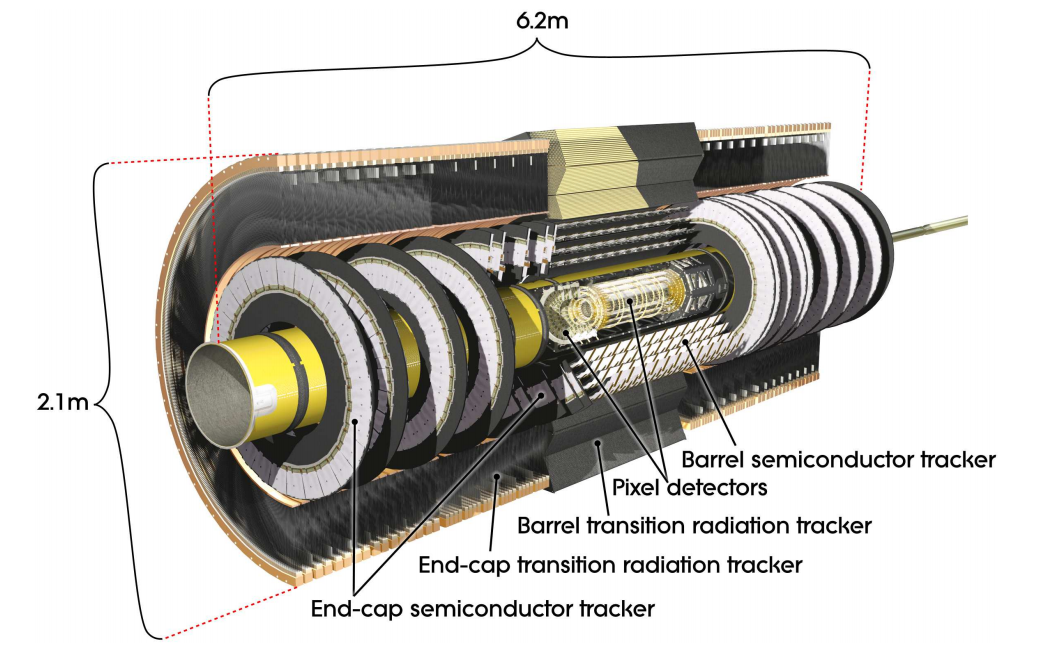
\includegraphics[width=0.8\columnwidth]{../ThesisImages/LHCImages/ATLASInnerDetector.png}
	\caption[Schematic of the ATLAS inner detector.]{Schematic of the ATLAS inner detector\cite{ATLAS}.
	}
	\label{fig:ATLASInnerDet}
\end{figure}

The IBL was added during Long Shutdown I (2016) of the LHC and is closer to the interaction point than the innermost layer in Run 1.  This required adding a smaller beam pipe (reduction in radius from 29mm to 25mm) but was able to improve the resolution of verticies and thus the reconstruction of events involving bottom quark decays as well as allowing for charm quark decays to be classified better than ever before.  This improvement is shown in Figure \ref{fig:impParamIBL} in a study of the impact parameter resolution.  An improvement of up to $40\%$ is seen with the inclusion of the IBL in the low $p_T$ region.  The IBL functions as a fourth layer of the Pixel Detector and uses planar sensors (similar to the Pixel Detector) as well as 3D sensors allowing electrons to interact with the bulk of the sensor as opposed to just the surface. 

\begin{figure}[ht!]
	\centering
	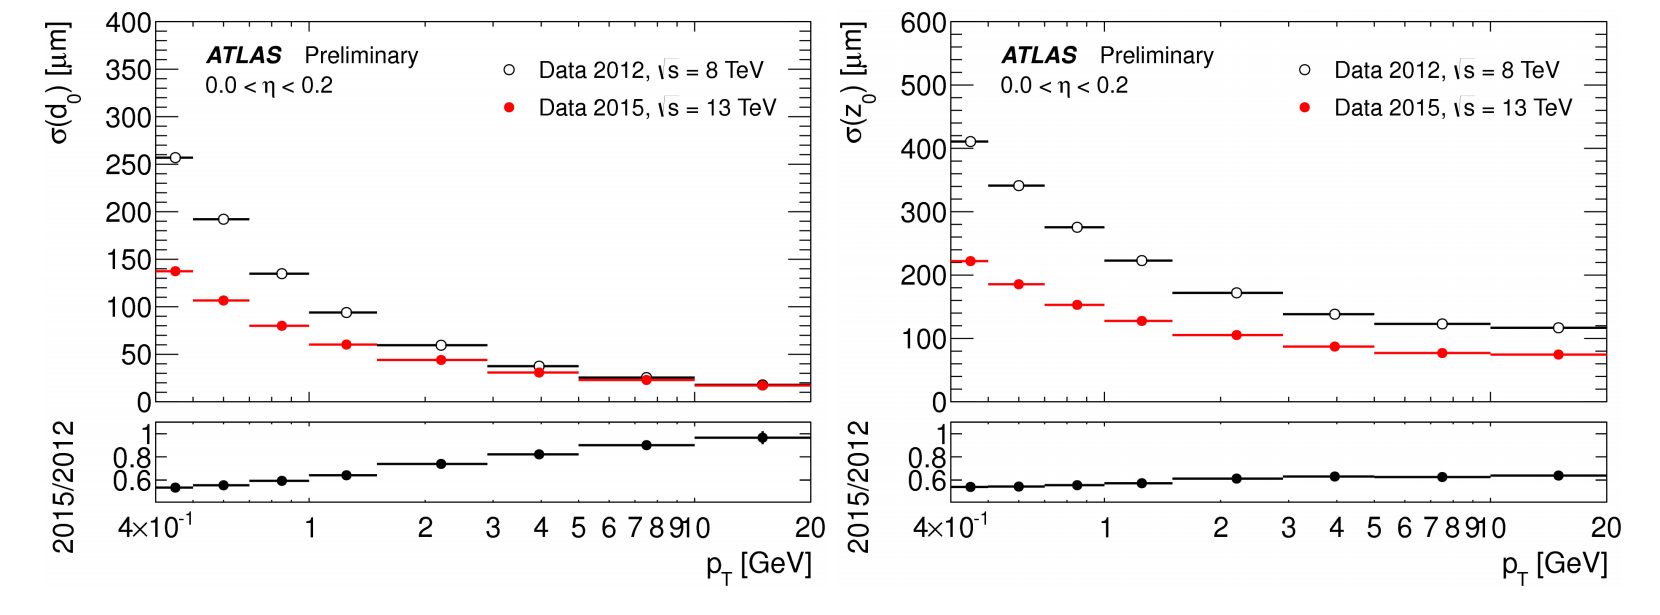
\includegraphics[width=\columnwidth]{../ThesisImages/LHCImages/tracking.png}
	\caption[Unfolded transverse (left) and longitudinal (right) impact parameter resolutions measured with (Run 2) and without (Run 1) the IBL as a function of $p_T$.]{Unfolded transverse (left) and longitudinal (right) impact parameter resolution measured with (Run 2) and without (Run 1) the IBL as a function of $p_T$\cite{Takubo:2017wvt}.
	}
	\label{fig:impParamIBL}
\end{figure}

The next layer from the beam pipe, as detailed in Figure \ref{fig:ATLASInnerDet}, is the Pixel Detector which is a series of high granularity silicon pixel detectors which measure a position when a charged particle passes through them.  These silicon pixels are n-doped silicon wafers biased with a high voltage that allow for the creation of electron hole pairs.  The electron then drifts toward the electrode which creates the position signal in the readout electronics.  In addition to the IBL there are three more cylindrical layers which are designed to ensure single pixel isolation and minimize leakage.  The pixels are $50 \times 400\mu\text{m}^2$.  For complete coverage to the cylindrical system, endcaps are placed on each side of the central barrel.  These endcaps consist of four wheels that have trapezoid shaped silicon pixels.  The three barrel layers consist of 67 million pixels and the endcaps total an additional 13 million pixels.
After the Pixel Detector is the Semiconductor Tracker (SCT) which is also made up of barrel and endcap detecors.  The barrel SCT is four cylindrical layers of silicon microstrip trackers where the endcaps are nine discs on each side of the barrel made up of either silicon or galium arsenide semiconductors.  The SCT contains over $60\text{m}^2$ of silicon detectors with over 6 million readout channels.

\begin{figure}[ht!]
	\centering
	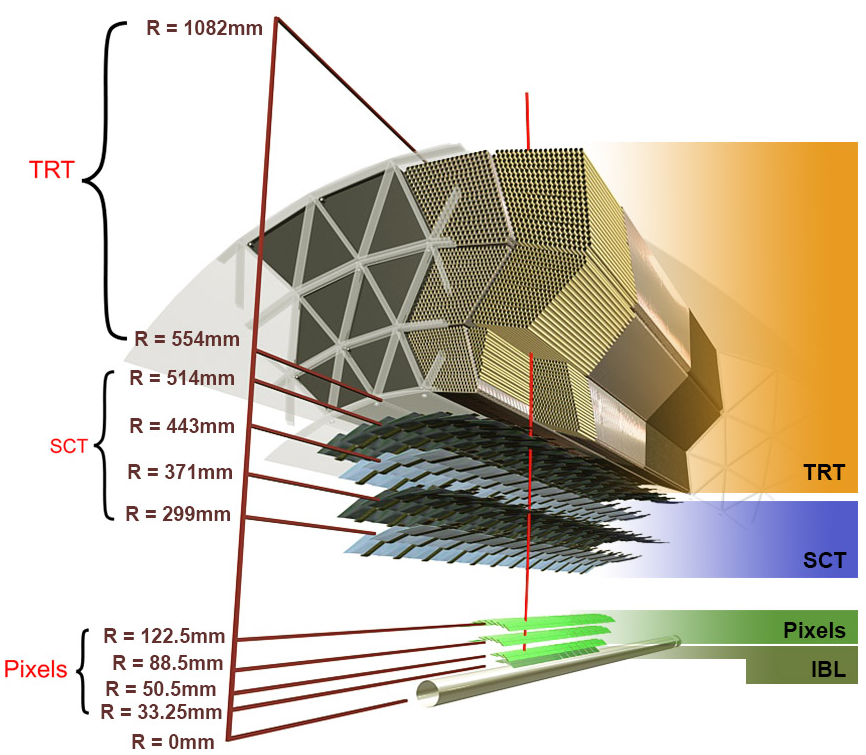
\includegraphics[width=0.5\columnwidth]{../ThesisImages/LHCImages/ATLASInnerStructure.png}
	\caption[Blown up schematic of the ATLAS inner detector with more detail.]{Blown up schematic of the ATLAS inner detector with more detail\cite{Potamianos:2016ptf}.
	}
	\label{fig:ATLASInnerDet}
\end{figure}

The final part of the Inner Detector is the Transition Radiation Tracker (TRT) \cite{Mindur:2017nqn}.  The TRT is a straw detector surrounding the SCT.  Every straw is a 4 mm in diameter Kapton tube with a 0.03 mm diameter gold-plated tungsten wire in its center.  In the barrel region there are 50,000 straws that are each 144 cm long and an additional 250,000 straws in both endcaps which are 39 cm in length.  Each straw is filled with an active gas mixture made up of mostly Xenon or Argon. 

When charged particles traverse across the TRT straws they ionize the active gas mixture and produce ionization clusters.  The amount of clusters created depends on how far the charged partcile traveled through the TRT (5-6 clusters per mm).  The straw walls are held at a high negative voltage such that the primary electrons are accelerated toward the gold-plated tungsten wire anode creating more ionization by liberating more electrons from the active gas and producing a detectable signal which is amplified and read out.  Transition radiation occurs when a particle makes a transition between materials with different dielectric constants and the energy radiated is directly proportional to the Lorentz factor of the particle.  This allows for an excellent discrimination between electrons and charged pions.



\subsection{Electromagnetic and Hadronic Calorimeters}
\label{sec:EMHCal}
While the inner detector focuses on tracking the charged particles as they pass through the detector the ATLAS Calorimeter system is designed to absorb and measure the energy of neutral and charged particles.  The exceptions to this are muons which are able to penetrate through the calorimeters into the muon and neutrinos which do not interact at all within the ATLAS detector.  The calorimeters can be broken down into two major systems, the Liquid Argon (LAr) calorimeter\cite{CERN-LHCC-96-041} and the tile calorimeter (TileCal)\cite{CERN-LHCC-96-042}.  Both of these systems are shown in Figure \ref{fig:ATLASCaloSys}.

\begin{figure}[ht!]
	\centering
	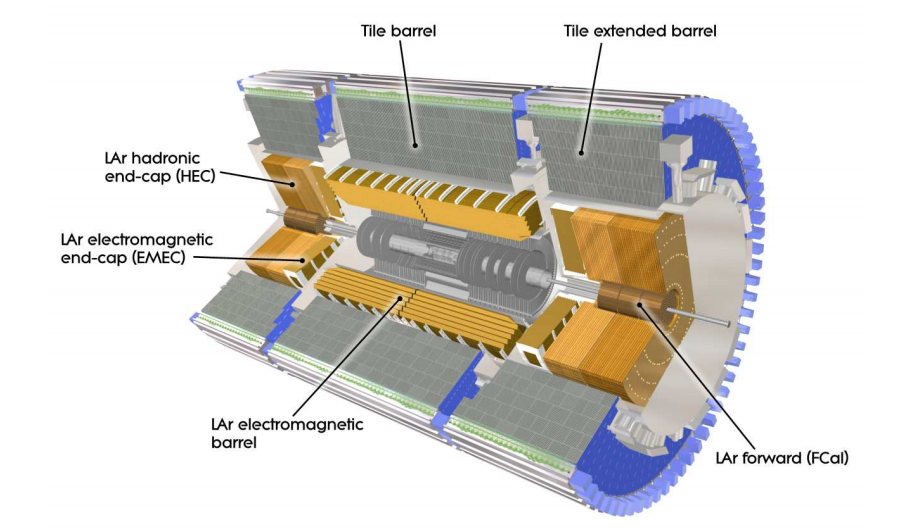
\includegraphics[width=\columnwidth]{../ThesisImages/LHCImages/ATLASCaloSystem.png}
	\caption[Schematic of the ATLAS hadronic and electromagnetic calorimeter systems.]{Schematic of the ATLAS hadronic and electromagnetic calorimeter systems\cite{ATLAS}.
	}
	\label{fig:ATLASCaloSys}
\end{figure}

The LAr calorimeter is a sampling calorimeter.  Sampling calorimeters use alternating layers of a dense absorbing material and an active material to measure the signal produced by showering particles.  The LAr calorimeter uses lead as the absorbing material and liquid argon measured with copper-tungsten sensors as the active layer.  The layers in the LAr calorimeter are arranged in an "accordian-shaped" geometry shown in Figure \ref{fig:LArAccordian} to provide complete azimuthal coverage.  This allows for the electromagnetic energy resolution to be uniform in the azimuthal direction.  Sampling calorimeters do not directly measure the entire energy of the particle, only the interactions that occur in the active layers. The stochastic nature of the processes being measured means that large fluctuations can occur while measuring electromagnetic showers.  These flucuations mean that sampling calorimeters must account for sampling statistics as opposed to other types of calorimeters where the entirety of the energy is absorbed with an active layer, such as scintillators.  
\begin{figure}[ht!]
	\centering
	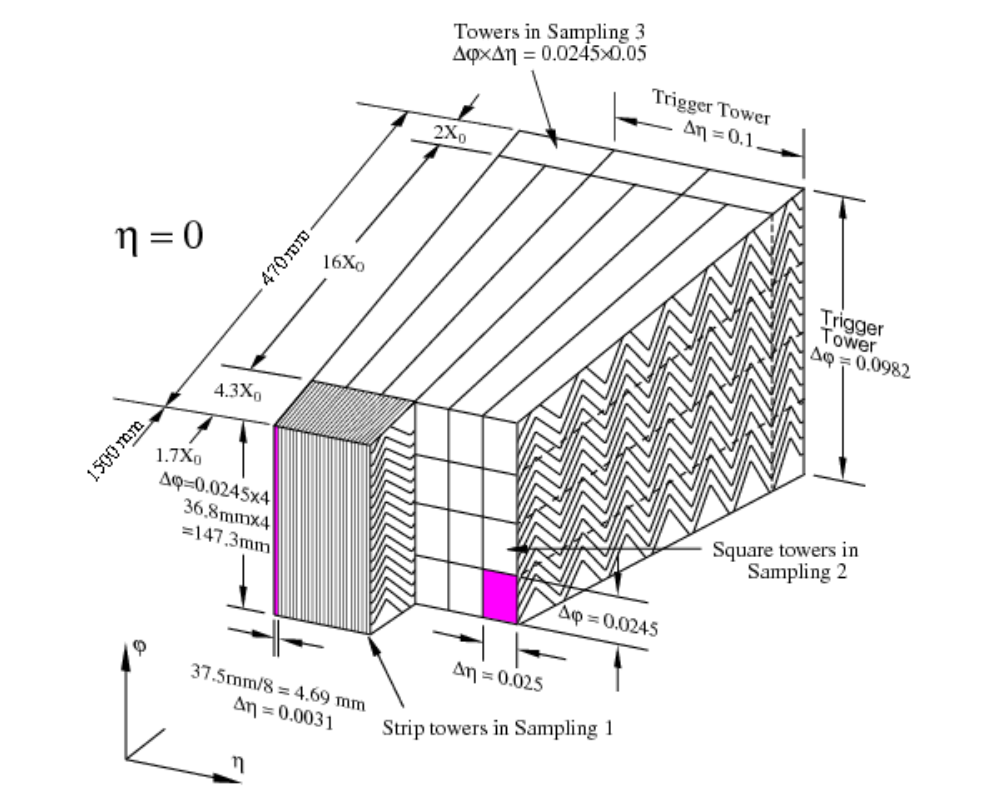
\includegraphics[width=0.5\columnwidth]{../ThesisImages/LHCImages/LArAccordian.png}
	\caption[Sketch of the accordian structure used in the LAr Calorimeter.]{Sketch of the accordian structure used in the LAr Calorimeter\cite{CERN-LHCC-96-041}.
	}
	\label{fig:LArAccordian}
\end{figure}

For sampling calorimeters it is important to know the ratio $\frac{E_{\text{visible}}}{E_{\text{deposited}}}$ so that the energy of a particle can be reconstructed based on only the energy measured by the active layers.  This ratio must be measured with test beams where the original beam energy is known precisely.  Sampling calorimeters allow for the complete detection of electromagnetic showers.  Because there is a large amount of material to traverse through, all of the energy can be deposited within the detector. The amount of material travesed by each particle is an important aspect as it includes not only the active material and absorber but also the support structures and cables that can play a role in particle interactions.  The thickness of a material passed through is typically measured in radiation lengths ($X_0$), where an electron passing through one radiation length will lose 1/e of its energy to bremsstrahlung.  The amount of radiation lengths in the LAr calorimeter is shown in Fugre \ref{fig:MaterialBudget}.  

\begin{figure}[ht!]
	\centering
	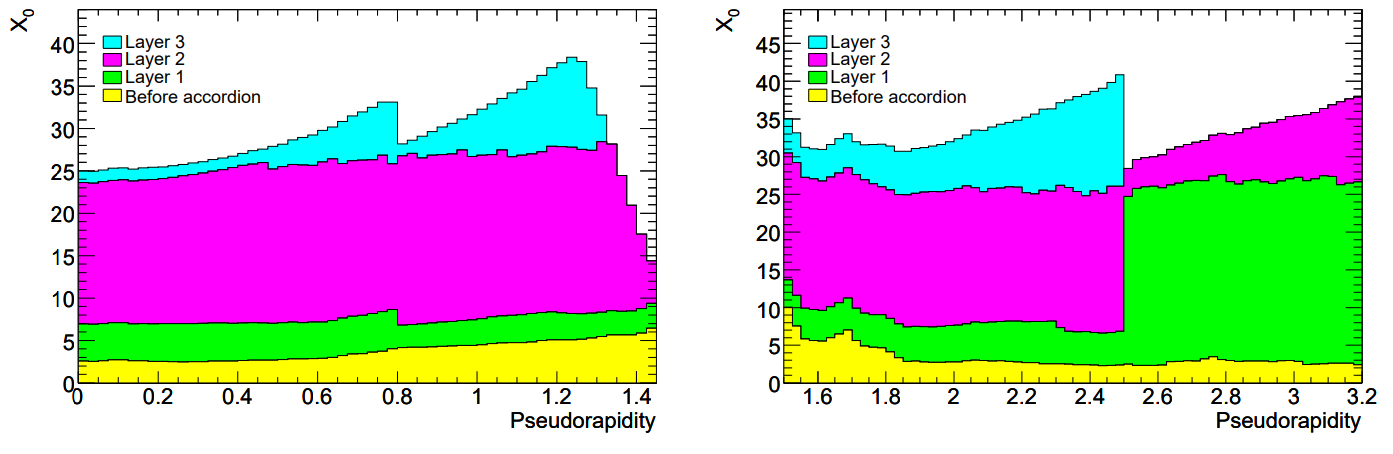
\includegraphics[width=\columnwidth]{../ThesisImages/LHCImages/MaterialBudget.png}
	\caption[Number of radiation lengths throughout the LAr calorimeter as a function of $|\eta|$.]{Number of radiation lengths throughout the LAr calorimeter as a function of $|\eta|.$\cite{ATLAS}
	}
	\label{fig:MaterialBudget}
\end{figure}

Forward from the barrel there are two electromagnetic endcap (EMEC) wheels with a similar accordion structure to the modules in the barrel that cover ranges $1.4<|\eta|<2.5$ and $2.5<|\eta|<3.2$.  Outside of the EMEC wheels is the LAr hadronic endcap (HEC) with a simpler parallel plate structure.  The last part of the LAr calorimeter is the LAr forward calorimeter (FCal).  Due to the FCal's proximity to the beamline the particle flux is very high so a dense calorimeter is used to avoid losing energy into other pieces of the detector.  The FCal is made up of three layers: the first is copper and the others are tungten.  

The remaining calorimeter system is the TileCal which is primarily responsible for hadronic calorimetry in the central region $|\eta|<1.7$.  TileCal is also a sampling calorimeter with iron plate absorbers and plastic scintillating tiles. The scintillating tiles are placed orthogonal to the beamline and readout using wavelength shifting fibers connected to photomultiplier tubes on the outside of the system.  TileCal has a fixed central barrel and two extended barrel sections as shown in Figure \ref{fig:ATLASCaloSys}.  The extended barrel sections can be moved.  The total nuclear interaction length of the TileCal is $7.4\lambda$, where $\lambda$ is the mean distance a hadronic particle will travel before experiencing an inelastic interaction with the material it is traveling through.  The total interaction length for each section of the calorimeter is shown in Figure \ref{fig:InteractionLengths}.


\begin{figure}[ht!]
	\centering
	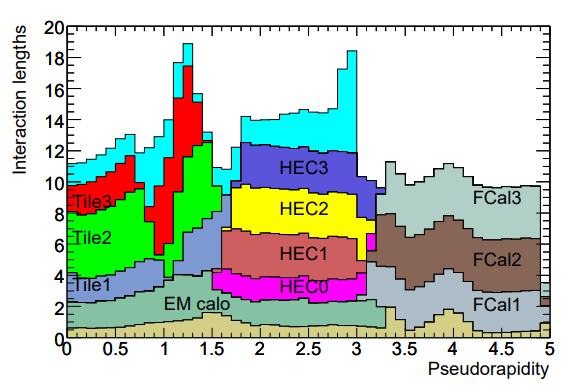
\includegraphics[width=0.8\columnwidth]{../ThesisImages/LHCImages/InteractionLengths.png}
	\caption[Number of interaction lengths throughout the LAr calorimeter as a function of $|\eta|$.]{Number of interaction lengths throughout the LAr calorimeter as a function of $|\eta|$.
	}
	\label{fig:InteractionLengths}
\end{figure}


\subsection{Muon System}
\label{sec:MuCal}
The final and outermost subdetector of the ATLAS detector is the muon spectrometer, which measures the momentum of muons.  Different technologies are used in the barrel and endcap regions for both measurement and triggering (deciding which events to keep when only a small fraction of events can be recorded).  For the barrel region, $|\eta|<2.7$, three layers of Monitored Drift Tubes (MDT) are used for precision energy and tracking measurements and Resistive Plate Chambers (RPC) for triggering.  In the forward region, $2.0<|\eta|<2.7$ , where the flux is higher, Cathode Strip Chambers (CSC) are used for energy and position measurements, and Thin Gap Chambers (TGC) are used for triggering.  These systems, shown in Figure \ref{fig:ATLASMuonSys}, are aided by the magnetic field created by the toroid system discussed in Section \ref{sec:ATLASMagnet}.
\begin{figure}[ht!]
	\centering
	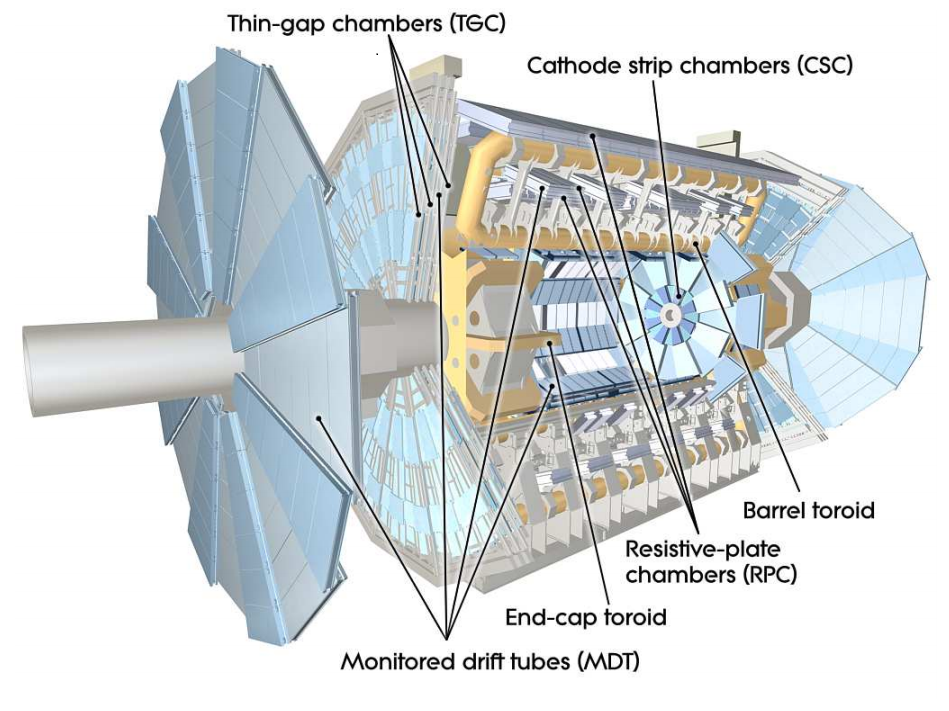
\includegraphics[width=\columnwidth]{../ThesisImages/LHCImages/ATLASMuonSystem.png}
	\caption[Schematic of the ATLAS muon detector.]{Schematic of the ATLAS muon detector\cite{ATLAS}.
	}
	\label{fig:ATLASMuonSys}
\end{figure}

MDTs are arranged in chambers of up to 6 layers of aluminum tubes ranging in length from one to six meters.  Each tube is 30 mm in diameter and contains a sense wire $50\mu\text{m}$ in diameter.  The chambers are arranged with a support spacer in between layers of MDTs that have a built-in optical sensor to monitor the drift tubes (hence the name) for deformations.  This ensures that the precision of measurements does not change over time.  The MDTs are only used in the barrel and not in the forward region because they are inappropriate in areas with high rates, in this case a high flux of muons. 

For the forward region CSCs are used.  CSCs consist of arrays of positively charged wires crossed with negatively charged strips within a gas.  As muons pass through they knock electrons from atoms in the gas which go toward the anode wires. Since the strips and wires are perpendicular to each other two position coordinates are read out.  CSCs have the benefit of giving acceptable one and two track resolution in a high flux environment.

The trigger system for muons in the barrel region uses RPCs which are parallel plates with opposite charges separated by a gaseous volume. A muon passing through an RPC knocks electrons from the gas which cause an avalanche of electrons that get picked up by the external metal strips rather than by the electrode.  The pattern of metal strips that gets hit gives a quick measurement of the muon momentum which is used by the trigger to make the immediate decision about the event.
The endcap muon trigger relies on TGCs.  TGCs are anode wires with graphite cathodes in between thin layers of fiberglass laminate.  Similarly to why CSCs are used over MDRs in the forward region TGCs have excellent timing resolution and can handle the high flux of muons in the forward regions.


\subsection{Trigger and Data Acquisition}
\label{sec:TDAQ}
The amount of data the LHC is capable of producing is staggering, and the ATLAS trigger system is required to reduce the enormous amount of data produced to a reasonable amount while keeping the most interesting events.  The LHC provides collisions at a rate of 40MHz.  Every event saved to tape requires about 1.6MB of space \cite{Outreach:1457044}. To keep all of the data produced 64TB/s would need to be saved or 230PB of data for a 12-hour run or 400EB of data per year (150 days of uptime). 

In order to reduce this to a manageable level the ATLAS trigger system uses a two level trigger system.  A hardware trigger, Level 1 or L1 trigger, is used to lower the rate from 40MHz to between 75 and 100kHz which is sent to the next level of the trigger system, the High Level Trigger (HLT).  Another factor of 50 in rate reduction is achieved by this software based HLT to reduce the rate below 2kHz.  A flowchart of the ATLAS trigger and data acquisition system is shown in Figure \ref{fig:ATLAStdaq}.  When combined with partial event readouts and the $<$2kHz full event readout the total bandwidth requirement is around 3GB/s to be written.  This means that only around $0.004\%$ of data is stored.
\begin{figure}[ht!]
	\centering
	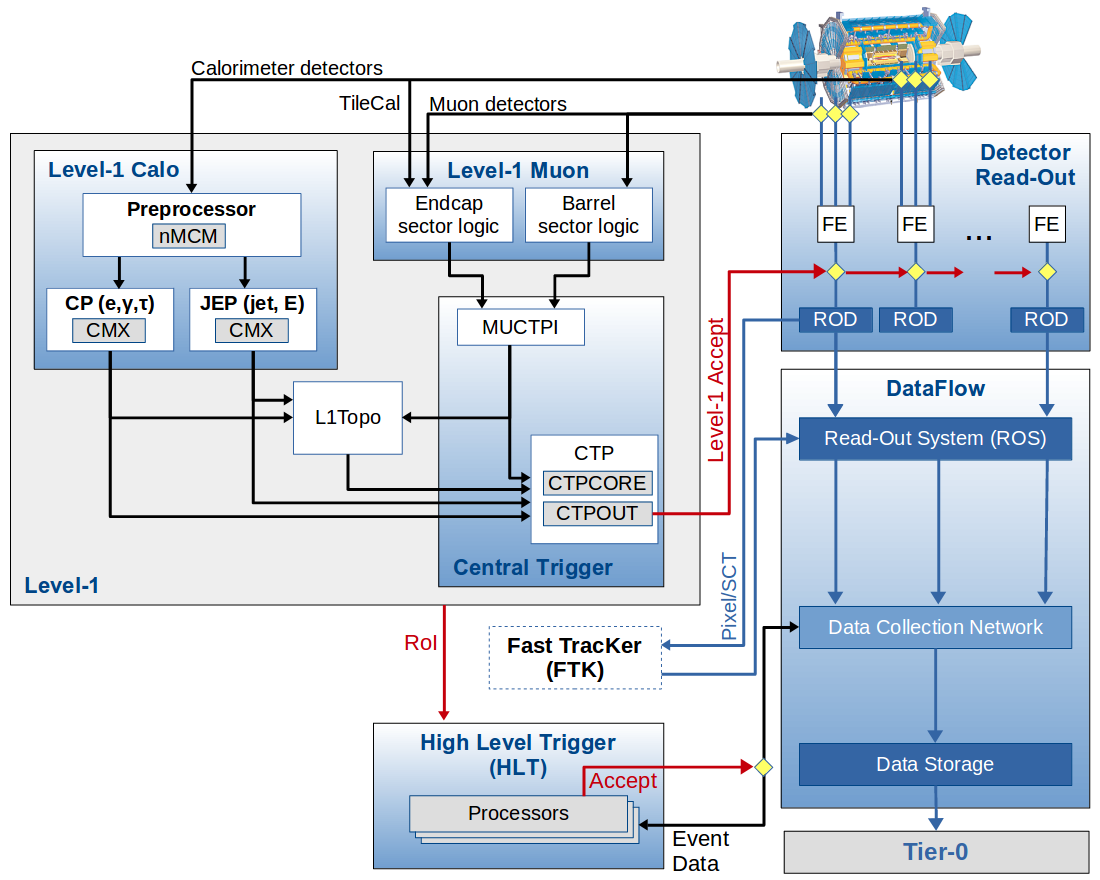
\includegraphics[width=\columnwidth]{../ThesisImages/LHCImages/ATLASTDAQR2.png}
	\caption[Flow diagram of the ATLAS trigger and data acquisition system used in Run 2.]{Flow diagram of the ATLAS trigger and data acquisition system used in Run 2\cite{ATLASTDAQ}.
	}
	\label{fig:ATLAStdaq}
\end{figure}

\subsubsection{Level 1 Calorimeter}
The Level 1 hardware trigger uses geometrically coarse information from some of the subdetectors.  The data from the calorimeters is sent to the Level 1 Calorimeter (L1 Calo) system.  L1 Calo uses low granularity information to identify Regions of Interest (RoIs) from objects that interact in the calorimeters (e.g., photons, electrons, jets, taus), events with high total energy, as well as events with an imbalance of energy coming from missing transverse energy.  The information is fed into the L1 Calo system and through a preprocessor that allows L1 Calo to handle the effects within ATLAS from pileup events.
Data from TileCal and the trigger portions of the muon systems goes to the Level 1 Muon (L1 Muon) system which applies various logical processes to determine whether or not an event should be kept.  
Outputs from L1 Calo and L1 Muon are passed to the Central Trigger Processor (CTP) which provides a level 1 trigger accept and LHC timing information to the detector read out.  At the same time the CTP gives RoIs to the HLT.

\subsubsection{High Level Trigger}
The HLT takes RoIs from the CTP as well as full detector granularity and makes a further decision whether or not that event should be saved.  This is done using a computing farm of over 40,000 cores that run over 2,500 independent algorithms (trigger chains) on the RoIs.  The HLT can provide partial and full event reconstruction depending on the event stream the event is decided to be within.  The main event stream is the physics analysis stream which gets full event reconstruction, while the other streams typically only require partial event reconstruction.  The other streams are used for a variety of things such as trigger level analysis, monitoring of the subsystems, and calibrating the detector.














